% ICRA 2027 submission — working title "Access Is Not Use" (08-06 사용자: 타이틀에 "loss" 미사용,
% loss 축은 본문에서도 디강조 — see NOTES.md)
% Compile on Overleaf (no local LaTeX). IEEEtran conference, 8 pages incl. references, double-anonymous.
% All numbers trace to Research/Paper_writing/FiLM/EVIDENCE.md (section refs in % comments).
\documentclass[conference]{IEEEtran}
\IEEEoverridecommandlockouts

\usepackage{cite}
\usepackage{amsmath,amssymb,amsfonts}
\usepackage{graphicx}
\usepackage{booktabs}
\usepackage{multirow}
\usepackage{makecell}
\usepackage{xcolor}
\usepackage{pgfplots}
\pgfplotsset{compat=1.17}
\usepgfplotslibrary{groupplots}
\usepackage[hidelinks]{hyperref}
% Local builds with tectonic (XeTeX): IEEEtran selects Times (ptm), which XeTeX has no
% TU-encoded shapes for; substitute the metric-compatible TeX Gyre Termes so pagination
% matches the pdfLaTeX/Overleaf build. No effect under pdfLaTeX.
\usepackage{iftex}
\ifXeTeX
  \usepackage{fontspec}
  \setmainfont{texgyretermes}[Extension=.otf, UprightFont=*-regular, BoldFont=*-bold,
    ItalicFont=*-italic, BoldItalicFont=*-bolditalic]
\fi
% --- notation ---
\newcommand{\chat}{\ensuremath{\hat{c}}}
\newcommand{\Fmag}{\ensuremath{\lVert F\rVert}}

\begin{document}
\bstctlcite{IEEEexample:BSTcontrol}

% 09-14 (사용자): 구조 위주 재프레이밍 — 워킹 타이틀. 구 "Access Is Not Use" 는 NOTES.md 참조.
\title{Grounded Force Conditioning for Behavior-Cloned VLA Policies:\\A Drop-In, Retrofittable FiLM Pathway That Brakes Beyond the Demonstrations}

% Double-anonymous: no author block content until camera-ready.
\author{\IEEEauthorblockN{Anonymous Authors}\\
\IEEEauthorblockA{Paper ID: XXXX}}

\maketitle

\begin{abstract}
% Abstract (~230 words). REWRITE 09-14 (사용자 결정): 구조(pathway) 위주 — 세 성질 drop-in /
% retrofittable / monotone-beyond-demos. π0.5 미언급 (사용자). 수치 출처 RESULTS_LINEUP + EVIDENCE §3.5, PI0 doc.
Vision-language-action (VLA) policies increasingly receive wrist wrench and contact signals in
their state, yet a behavior-cloned policy given the full wrench can still fail to bind its
behavior to it. On a real-robot suction case-picking task where the cases carry battery
cells---a $15$\,N contact-force limit, and a stop-on-contact transition observable only through
force---a naively fine-tuned VLA presses through contact in every trial and never stops on its
own. We present a conditioning pathway that changes how force is delivered, not what is
delivered: a condition vector \chat{} (contact, force magnitude, seal) computed from signals the
policy already receives, injected by FiLM at the state token, with the raw wrench masked. The
pathway has three properties. It is \emph{drop-in}: no backbone change, no new information, no
cost in imitation error, and it attaches to a second backbone ($\pi_0$). It is
\emph{retrofittable}: added to an already-trained naive policy, a few thousand steps of
continued training suffice. And it \emph{extrapolates in the right direction}: because \chat{} is a
calibrated monotone scalar, the policy brakes harder the harder it is pressed---stopping and
retreating at forces beyond the demonstrations, where the naive policy's response fades---and
picks succeed at a stack height absent from training. A matched ablation shows both
ingredients are necessary: unmasked, the pathway trains causally dead (\emph{bypass});
ungrounded, it is the worst policy in the study. We also ran it on our robot: every
conditioned pick stops on its own (median contact force $2.5$\,N) where the naive policy is
externally aborted in every attempt, and on-robot counterfactual probes reproduce the offline
crossover.

\end{abstract}

\begin{IEEEkeywords}
imitation learning, vision-language-action models, force control, causal confusion, contact-rich manipulation
\end{IEEEkeywords}

% §I Introduction (~1.0 page, Fig. 1). REWRITE 08-11 (사용자 결정): prescription-led arc —
% problem → cause (bypass) → recipe (grounded bottleneck + decorrelated demos) → thesis.
% Thesis = crossover: "indistinguishable in loss, similar at demonstrated forces, categorically
% different exactly where the task is decided." Quintuple recast as ablation of the recipe.
% Robot evidence in force language (contact-force distributions, censoring); success counts
% deferred to §VI and subordinated there. Nugget sentence PROMOTED here from old §VI closer —
% §VI rewrite must not repeat it verbatim.
% Forbidden narratives respected: no "naive is force-blind" (state-transplant 105%); scope
% limited to correlated-BC + existing shortcut (토론 1/5). All numbers EVIDENCE §3, 0729-pure.
% Terminology 08-11 (사용자): unconditioned policy = "naive policy" (defined at first mention
% with "full wrench in its state"), replacing "baseline" PAPER-WIDE — rename §III–§VII prose
% and table labels ("naive VLA (full wrench)") as each section is rewritten.
\section{Introduction}
\label{sec:intro}

Behavior-cloned vision-language-action (VLA) policies are rapidly acquiring physical condition
signals. Wrist force/torque, contact events, and task-state bits now routinely appear in the
observation vector, and a growing line of work fuses force into the policy backbone for
contact-rich manipulation~\cite{forcevla,phaforce,forceflow,filic}. All of this work shares a
validation recipe---add the signal, retrain, and validate by task success (occasionally
alongside rollout force statistics~\cite{phaforce,forceflow})---and none of it measures
whether the trained policy \emph{causally uses} the signal when it matters: whether, holding
everything else fixed, changing the force input changes the action. Imitation learning offers no
such guarantee. The objective asks the policy to reproduce \emph{what} the expert did, not
\emph{why}: a clone can imitate the behavior convincingly while being driven by entirely
different cues than the expert was. Imitation pins down the trajectory, not the
mechanism---equally faithful clones can act from opposite causes, and the loss cannot tell
them apart~\cite{dehaan2019causal,geirhos2020shortcut}.

The consequence is easiest to see where force is the only signal that can carry the task. We
study real-robot suction case picking with a single head-mounted camera and no wrist camera: the
arm must stop descending the moment the suction cup meets the case, and stack heights differing
by a few millimeters---the entire success margin---are visually near-indistinguishable at
head-camera range. The wrench is in the state the policy receives, and every demonstration
exhibits the stop. Yet a naively fine-tuned VLA---full wrench in its state, hereafter the
\emph{naive policy}---presses through contact in every evaluation trial and never initiates a
stop of its own: each run ends only when an external safety layer, separate from the policy,
trips at its $15$\,N force limit---set to protect the battery cells the cases carry
($15.4$--$18.7$\,N measured at abort)---the policy still commanding descent. The task turns on a single transition---stop when force
rises---and it is precisely this transition that the policy fails to bind to force.

Our fix changes how force is delivered, not what is delivered. A condition vector \chat{}
(contact, normal force, seal) is \emph{computed} from signals the naive policy already receives
and injected through FiLM modulation~\cite{perez2018film}; the raw wrench is masked from the
state so that the same signal does not enter twice, making \chat{} the \emph{only} pathway from
force to action. We call this pathway \emph{grounded} because its content is computed from
measured signals, and the policy trained behind it the \emph{conditioned policy} (``FiLM
(ours)'' in tables and figures). By
construction it receives no information the naive policy lacks, and because the pathway is
explicit and unique, forcing \chat{} at inference directly measures its \emph{causal
authority}---the fraction of commanded descent the condition can cancel.

The mask is load-bearing. Leave the raw wrench in the state and the conditioning pathway trains
causally dead at unchanged validation loss: training routes force through the already-functional
raw path and starves the dedicated one. We call this \emph{bypass} and exhibit it in
Sec.~\ref{sec:offline}; it is why a fix of this kind cannot be certified after the fact, and why
ours holds by construction. The demonstrations complete the recipe: each press-retreat episode
presses to a randomized force target and retreats before any seal event, so the force at which
the expert stops varies from episode to episode---in the data, depth, appearance, and timing no
longer predict the stop; only the force reading does. The same interface that fixes the policy
is the instrument that audits it (Sec.~\ref{sec:method}).

The resulting policy is not uniformly better---it is different exactly where the task is
decided. In a matched comparison---same data, same initialization, imitation error
indistinguishable---the naive policy \emph{does} respond to force at the demonstrated
magnitudes, as strongly as the conditioned policy or more so. But its response is a
\emph{template}: sized to the demonstrated forces, it fades or saturates as force rises past
them, never strengthening into a stop. The conditioned policy's response instead grows with
force, to the point of stopping and
backing away at forces beyond anything in the training data (Sec.~\ref{sec:offline}). The
mechanism carries to the real closed loop: while the naive policy drives contact force past the
$15$\,N safety limit on every attempt, the conditioned policy stops on its own in every
pick---across three stack heights, at a median contact force of $2.5$\,N---and live
counterfactual probes reproduce the offline crossover on the physical system
(Sec.~\ref{sec:robot}).

Our contribution is the pathway and three properties of it, each measured by intervention on
the trained policy (Sec.~\ref{sec:method-probes}):
\begin{itemize}
\item \textbf{Drop-in.} \chat{} is computed from signals the policy already receives and
  enters through an identity-initialized FiLM layer at the state token; the backbone is
  untouched, no information is added, imitation error is unchanged, and the same pathway
  attaches to a second backbone ($\pi_0$), where it again turns a policy that never stops into
  one that does (Sec.~\ref{sec:method},~\ref{sec:offline-pi0}).
\item \textbf{Retrofittable.} Added to an already-trained naive policy and continued for a
  few thousand steps on the same demonstrations, the pathway turns a saturating force template
  into a monotone brake; a matched ablation shows the mask and the grounding are both
  necessary---unmasked, the pathway trains causally dead (\emph{bypass}); ungrounded, it is the
  worst policy in the study (Sec.~\ref{sec:offline}).
\item \textbf{Monotone beyond the demonstrations.} Because \chat{} is a calibrated monotone
  scalar, braking grows with force past anything demonstrated, stopping and retreating where
  the naive policy's template saturates and presses through (Sec.~\ref{sec:offline}). The
  same holds on our robot: every conditioned pick stops under the $15$\,N abort limit (median
  contact force $2.5$\,N), including at a stack height absent from the demonstrations, and
  live counterfactuals reproduce the crossover (Sec.~\ref{sec:robot}).
\end{itemize}

\noindent In one sentence: \emph{a policy that stops when it feels what the demonstrations felt
and a policy that stops harder the harder it is pressed are indistinguishable in loss and
similar at the demonstrated forces---they differ exactly where the task is decided, and only
demonstrations in which force alone predicts the stop, behind a grounded, masked FiLM
pathway, yield the second.}

% §II Related Work (~0.75 page). 4 clusters per OUTLINE §5-II. Differentiation via 토론 1
% (3-layer claim discipline: their evidence doesn't establish causal use; ours is an existence
% proof of bypass; falsifiable prediction, not accusation).
% 08-11 reviewer-proofing (reference/ANALYSIS.md 전수조사 기반): near-miss 구분 추가 —
% TA-VLA(노이즈는 baseline 토큰, HSIC는 상관), Tactile-VLA(dose-response는 language 입력),
% ForceFlow(마스킹은 vision 입력), ForceSight(개입은 출력 force goal, readout은 SR).
% hedge "rollout force statistics" §I과 미러링. FuSe/FM-VLA = 분야가 인지하고도 SR로만 검증한 사례.
\section{Related Work}
\label{sec:related}

\textbf{Force- and tactile-conditioned VLA policies.}
ForceVLA fuses wrist force as dedicated tokens through a mixture-of-experts
backbone~\cite{forcevla}; TA-VLA injects torque adapters into the action
decoder~\cite{tavla}; PhaForce schedules policy phases on contact and force
signals~\cite{phaforce}; ForceFlow~\cite{forceflow}, FARM~\cite{farm}, and
FILIC~\cite{filic} condition diffusion or impedance-loop policies on force and tactile
input; TacForeSight learns force-conditioned tactile prediction~\cite{tacforesight}.
Each commits to a way of getting force into the network---new tokens, new experts, new
adapters, a new decoder---and each is validated by task success and retraining ablations,
sometimes alongside rollout force statistics~\cite{phaforce,forceflow}. Our pathway is the
lightest of these choices: a computed condition modulating the state token of an otherwise
unchanged backbone, attachable after training. We also evaluate differently: rather than
comparing differently trained policies by success, we intervene on the force input of a
trained policy and read the action, which exposes the \emph{form} of the response---whether
it grows or fades with force---that success rates average over. The closest such analyses
stop short of the force input: TA-VLA perturbs input tokens of its baseline~\cite{tavla},
Tactile-VLA's dose-response intervenes on the instruction~\cite{tactilevla}, and ForceFlow
masks its trained policy's visual input~\cite{forceflow}.

\textbf{Intermediate condition representations.}
Injecting a compact, task-level representation between observation and action is a recurring
design: RT-Affordance conditions on predicted affordance plans~\cite{rtaffordance}, and FiLM
modulation~\cite{perez2018film} is the standard mechanism for conditioning a backbone on side
information. Our \chat{} shares the shape but differs in role: it is computed from signals the
policy already receives rather than learned, so it adds no information and its meaning is fixed
before training.

\textbf{Causal confusion and shortcut learning.}
That imitators latch onto spurious correlates is well established: causal confusion in
IL~\cite{dehaan2019causal}, copycat behavior on observation histories~\cite{wen2020copycat},
and shortcut learning in deep networks broadly~\cite{geirhos2020shortcut,hermann2023foundations}.
Recent work documents shortcuts in generalist robot policies~\cite{shortcutgeneralist} and uses
targeted interventions to expose or correct them~\cite{interventionil2025,interventionil2023}.
The symptoms are on record in force-FiLM policies themselves: FuSe observes fine-tuned
generalists ignoring newly added sensors~\cite{fuse}, and FM-VLA diagnoses a history-length
shortcut in its own force stream and patches it with augmentation---verifying the fix, again,
only by task success~\cite{fmvla}.

\textbf{Privileged supervision and interventional evaluation.}
Privileged-teacher distillation~\cite{chen2020lbc,privilegedaction} assumes access to a signal
worth distilling; our probes instead ask how a deployed policy responds to the signal it already
has. The closest interventional precedent is ForceSight, which ablates predicted force
\emph{goals} at its controller under matched initial conditions~\cite{forcesight}; the
intervention sits on the output side of a model that takes no force input, and reads out
end-of-episode success rather than the action. Our press-retreat demonstrations are a data-side
decorrelation in the spirit of fixes for causal confusion~\cite{dehaan2019causal}, motivated
by a physical argument (Sec.~\ref{sec:discussion}).

% §III Task and the Failure (~0.75 page, Fig. 2). 0729-pure per Q2: no June depletion sweep /
% gate-oracle in body. Failure = naive 0/3 overpress (canonical: EVIDENCE §3 08-11 블록). The
% policy is phenomenologically described here; mechanism diagnosis deferred to §V (probes).
% 08-11 수정: 용어 naive policy로 통일; abort는 external-layer/censored 서술 (§I과 정합);
% 성공 카운트 미표기 ("every evaluation trial"). 로봇 명시 08-11 사용자 결정: Dexmate Vega-1p
% (하드웨어 벤더 명시는 double-anonymous 허용 관행; 필요시 camera-ready 전 재검토).
\section{Task, Setting, and the Failure}
\label{sec:task}

\textbf{Task and platform.}
We study suction case picking on a Dexmate Vega-1p, a dual-arm mobile manipulator: the arm
descends onto a stack of rigid cases, must stop when the suction cup meets the top case, hold
until vacuum seal is confirmed, and lift (Fig.~\ref{fig:setup}). The cases carry battery
cells, which tolerate little compression---over-pressing risks the product, not just the
pick---so deployment enforces a $15$\,N contact-force limit. The margin is tight in both
directions: too little press and the seal fails; a few millimeters too much and contact force
climbs past the limit, since the stack is stiff (${\sim}5$\,N/mm, Sec.~\ref{sec:discussion}). The policy
controls a 7-D end-effector action ($3$-D position and $3$-D rotation increments plus a
suction command) at $15$\,Hz, executed in chunks of $5$ actions (${\sim}330$\,ms between
observations).

\textbf{Observations.}
The policy observes a single head-mounted camera (RGB and colorized depth; no wrist camera) and a
15-D state: end-effector position and quaternion, suction command, vacuum-seal bit, and the 6-D
wrist wrench. The setting is a deliberately clean diagnostic: at head-camera range, case-stack
heights differing by millimeters---the entire success margin---are visually near-indistinguishable
(Fig.~\ref{fig:setup}, right), while the wrench and seal bit signal the contact transition
directly. Every condition the task depends on is \emph{in the state the policy receives}; the
question is whether the policy binds its behavior to it.

\textbf{Demonstrations.}
We collect $100$ training episodes ($19{,}445$ frames) and hold out $6$ validation episodes
($1{,}169$ frames) with a scripted expert designed to \emph{decorrelate} force from its habitual
correlates: each episode descends with suction on, presses to a randomized force target drawn
from $[8,15]$\,N, retreats $5$--$10$\,mm from the contact plane, then hovers and lifts
immediately on seal. Episodes are collected at two different stack heights, so the contact
plane itself moves across the dataset. Every episode thus demonstrates the counterfactual the task requires:
force rises $\rightarrow$ stop $\rightarrow$ move back up, \emph{before} any seal event, at a
force level that varies independently of depth. This is the data-side prescription whose
rationale we develop in Sec.~\ref{sec:discussion}; here it matters that the naive policy and
all conditioned variants are trained on exactly these episodes.

\textbf{The failure.}
Deployed on the robot, the naive policy---a SmolVLA~\cite{smolvla} fine-tuned on these
demonstrations, with the full wrench and seal bit in its state---fails every evaluation trial
the same way: it descends, makes contact, and keeps pressing---never initiating a stop of its
own---until the external safety layer aborts the run ($15.4$--$18.7$\,N measured at abort).
The transition that the demonstrations exhibit in every single episode, driven by the one signal
that observably announces it, is the transition the policy does not perform. The rollout says
the policy is bad; it does not say \emph{why}. The policy might ignore force entirely; it might
respond to force but too weakly; it might respond in a form that collapses precisely when force
exceeds the demonstrated range. These hypotheses have opposite prescriptions (more data?
different sensors? different architecture?), and none of them is distinguishable from training
curves or rollouts. Distinguishing them requires intervening on the signal itself---the
instrument we build next.

% §IV Instrument (~1.25 pages, Fig. 3). Terminology FIXED here (EVIDENCE 혼용 금지):
%   "condition-forcing probe" = synthetic c-hat forcing (std/realistic 계열)
%   "state-transplant probe" = measured first-contact state injection (state-swap 계열)
%   "dose-response sweep"    = fcscale ramp 8/10/12N
%   "press simulation"       = closed-loop probe_press_sim
%   "live counterfactual probe" = on-robot frozen-obs
% Authority = % of mean commanded descent cancelled by the intervention.
% 08-11 수정: 용어 naive policy 통일; 각주 = 인스턴스 공시 전담 (RESULTS_LINEUP D 가드레일 ②);
% 서두를 prescription 프레임에 연결 ("recipe의 구조 절반이 instrument를 겸한다").
\section{The Conditioning Pathway}
\label{sec:method}

The pathway has two parts: a conditioning route built so that force reaches the action in one
explicit, calibrated form (\ref{sec:method-chat}--\ref{sec:method-mask}), and a battery of
counterfactual probes that measure how much that route moves the action
(\ref{sec:method-probes}). The route is designed to be \emph{drop-in} (no backbone change, no new
information), \emph{retrofittable} (attachable to a trained policy), and \emph{measurable}: because
it is explicit and unique, every component makes one number well-defined---how much does the
condition causally move the action?

\begin{figure}[t]
\centering
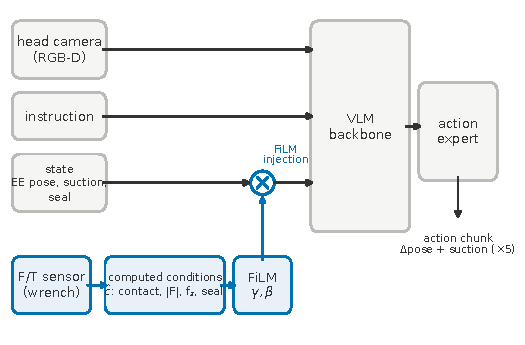
\includegraphics[width=\linewidth]{figs/architecture}
% 08-12 사용자 결정: mask는 그림에 미표기 — wrench가 state에 아예 없는 것으로 묘사
% (기능적으로 동등; mask 메커니즘은 §IV-C 본문이 설명).
\caption{The conditioned policy. The raw wrench does not enter the policy state; force reaches
the action only as the computed condition vector \chat{}, injected through FiLM modulation of
the state token entering the VLM backbone. Because this pathway is explicit and unique, forcing
\chat{} at inference measures the causal authority of the condition.}
\label{fig:arch}
\end{figure}

\subsection{Computed condition vector \chat{}}
\label{sec:method-chat}
From the wrench $F$ and seal bit already present in the naive policy's state we compute a small
set of task-critical conditions---the physical cues a human operator references (``if you feel
contact, stop; if the seal is on, lift''):
\begin{align}
\chat_{\mathrm{contact}} &= \mathrm{clip}\!\left(\left(\Fmag - F_0\right)/\tau,\ 0,\ 1\right),\nonumber\\
\chat_{\mathrm{fmag}} &= \left(\Fmag - F_0\right)/\tau_m \quad\text{(unsaturated)},\nonumber\\
\chat_{f_z} &= \left(f_z - o_z\right)/\tau_z,\qquad
\chat_{\mathrm{seal}} = \mathrm{seal},
\label{eq:chat}
\end{align}
with offsets and scales calibrated to the measured force statistics of the demonstrations (e.g.,
$F_0$ at the contact-onset magnitude).\footnote{Calibration quality matters and is itself a
finding. The conditioned policies in this paper are separately trained instances of the same
design: the robot picks (Sec.~\ref{sec:robot}) and the replication pair quoted in
Sec.~\ref{sec:offline-quintuple} use an earlier calibration; the recipe ablation and the live
counterfactuals (Sec.~\ref{sec:robot-live}) use offsets re-estimated from the measured contact
distribution plus the unsaturated $\chat_{\mathrm{fmag}}$ channel.} Two properties are essential. \emph{Computed, not
learned:} \chat{} is a fixed function of observed signals, so its physical meaning cannot drift
during training---which is what makes forcing \chat{} at inference a well-defined intervention
rather than a perturbation of an arbitrary latent. \emph{Zero new information:} every channel is a deterministic
function of state dimensions the naive policy also receives, so conditioning changes
\emph{routing}, never \emph{content}---the ``it works because it got extra sensing'' objection is
excluded by construction. The channels are deliberately plural: keeping contact, force magnitude,
and seal separate is what later lets the probes attribute authority to specific signals
(Sec.~\ref{sec:offline-posthoc}).

\subsection{FiLM injection and the force mask}
\label{sec:method-mask}
\chat{} enters the policy through FiLM modulation~\cite{perez2018film} at the state token
entering the VLM backbone; the injection site matters, and Sec.~\ref{sec:offline-pi0} compares
it against the action token.
% 09-15: "preliminary experiments" 각주 삭제 (사용자) — 근거는 §V-C π0 state vs action 비교로 대체.
The FiLM layer is zero-initialized so that it starts as the identity, and the backbone is
untouched: at the moment the pathway is attached, the conditioned policy \emph{is} the
already-trained policy, and can be fine-tuned in place from there. Every offline conditioned
policy in this paper is obtained this way, by continuing the trained naive checkpoint
(Sec.~\ref{sec:offline}).
The policy still receives the force information---only the structure of its delivery changes.
Because \chat{} is computed \emph{from} the wrench, leaving the raw wrench in the state would
hand the policy the same signal twice, once in each form; we therefore mask the wrench
dimensions from the state (Fig.~\ref{fig:arch}). Forcing \chat{} at inference then manipulates
\emph{all} of the force information the policy receives: if the policy responds to force at
all, it must show in how the action changes with \chat{}---the quantity the probes below
measure.

\subsection{Evaluation: counterfactual probe battery}
\label{sec:method-probes}
All probes intervene on a trained, frozen policy; none involves retraining. The offline probes
(P1--P4) run on held-out validation episodes. We define
\textbf{authority} as the intervention-induced change in the commanded vertical action on
committed-descent frames, expressed as a percentage of the mean commanded descent: $0\%$ means
the intervention is ignored, $100\%$ means it fully cancels descent, ${>}100\%$ means reversal
(retreat).

\textbf{(P1) Condition forcing (open loop).} How much does the condition alone move the
action? With images and state frozen, \chat{} is forced from its observed value to a target
pattern---either all channels saturated (\emph{full forcing}) or a calibrated contact-onset
pattern matching measured first-contact statistics (\emph{contact-moment forcing}). Applicable
to conditioned models only.

\textbf{(P2) State transplant (open loop).} Does the policy respond to a \emph{real}
contact state, and through which route? The six wrench dimensions of a measured first-contact
state (the median wrench at the first force rise, pooled over episodes; the seal bit keeps its
pre-contact value) are transplanted into pre-contact descent frames. This probe applies to any
policy, including the naive policy---it is what puts both policies on the same scale. Routing
the transplant selectively, to the \chat{} computation alone ($d_{\mathrm{FiLM}}$) or the raw
state alone ($d_{\mathrm{raw}}$), attributes the response to each route.

\textbf{(P3) Dose-response sweep.} Does the policy brake \emph{more} the harder it is
pressed? A policy that has bound braking to force should; one that has memorized a contact
template should respond most near the template and fade beyond it. The transplanted wrench is
rescaled to $8$, $10$, and $12$\,N and the response traced as a function of force \emph{dose};
since the demonstrations peak near the low end of this range, the upper doses measure
extrapolation. The sweep's \emph{slope sign} is the paper's central discriminator.

\textbf{(P4) Closed-loop press simulation.} Does the policy actually stop before the force
limit when no seal ever comes? Open-loop probes cannot show consequences, so we place the
frozen policy in a closed loop at each episode's nominal first-contact timing: commanded
descent advances a virtual penetration depth, a linear-stiffness force model raises the
simulated wrench accordingly, and the seal event is withheld---the operationally critical
misalignment scenario in which no press depth ever produces a seal. Outcomes: whether the
policy stops before the force limit, and maximum penetration. A control variant grants the seal
at a shallow depth, separating force-driven stopping from seal-event-driven stopping.

\textbf{(P5) Live counterfactual probe.} Do the offline responses hold on the real robot,
where the sensor, the contact, and the control loop are real rather than replayed or
simulated? We freeze observations at staged poses
along the approach and apply (P1)--(P3) interventions to \emph{two} policies---the conditioned
policy and the naive policy---on identical frozen observations, so both receive the same
physical counterfactual.

\textbf{Scope.} P1--P3 are single-frame and open-loop; P4 closes the loop under a force model;
P5 closes the gap to the real system. No single probe is decisive---the findings below rest on
their agreement.

% §V Experiments — offline battery. REWRITE 08-11 (RESULTS_LINEUP.md A1–A3, 보고 정책).
% 08-11 결정: best-only 보고 (균일 규칙, 서두 선언); 용어 naive policy. 09-14: fig:doseresponse = figs/dose_response.tex (pgfplots, 스크립트 생성).
% 08-12 압축 (사용자): bypass 소절 + Table I 삭제 (유지).
% 08-12 재구성 (사용자): ① 결과 제시 probe 순서 P1→P4 (P5는 §VI-B) ② 표/서사 분리 —
%   §V-A = naive vs conditioned 2행 표 (tab:probes), §V-B = ablation 컨트롤 2행 표
%   (tab:ablation; wrench-kept/shuffled + bypass·grounding-not-capacity 문단).
%   P1 수치 출처 (fromnaive 라운드, val ep0 — probe_film_authority.py 헤더의 "training data"는
%   stale 라벨): 0729_{fromnaive_best,mask0fn_main,v1_main}_std.txt COMMITTED-desc Δdz.
%   P1은 mm만 보고 (% 금지: P1 분모 −7.8mm/frame ≠ P2 분모 −1.7mm/frame — % 병렬 오독 유발).
% 가드레일: "naive는 force-blind" 금지 (transplant 105%); 캘리브레이션 라운드 간 % 직접
% 비교 금지; 인스턴스 공시는 §IV 각주 전담. 로봇 배포 ckpt = val-best (사용자 확인 08-11).
\section{Experiments}
\label{sec:offline}

\begin{table*}[!t]
\caption{Offline battery. Upper rows: the naive policy vs.\ the conditioned policy (FiLM,
ours). Lower rows: ablation controls with the same initialization and data and one
ingredient removed. Entries are the change in commanded descent caused by the intervention;
percentages are relative to the policy's own descent on the evaluated frames (\% own; none for
P1, whose frames differ). Press sim = the seal-never press simulation. The naive policy has no
\chat{} to force (---).}
\label{tab:probes}
\centering\setlength{\tabcolsep}{4.5pt}
\begin{tabular}{llrrrr}
\toprule
Policy & Force access & \multicolumn{1}{c}{\makecell{Forcing (P1)\\{\scriptsize mm/frame}}} & \multicolumn{1}{c}{\makecell{Transplant (P2)\\{\scriptsize mm/frame (\% own)}}} & \multicolumn{1}{c}{\makecell{Dose-response (P3), $8\rightarrow12$\,N\\{\scriptsize mm/frame (\% own)}}} & \multicolumn{1}{c}{\makecell{Press sim (P4)\\{\scriptsize max depth (mm)}}} \\
\midrule
naive VLA   & raw wrench               & ---                     & $+1.63$ (105\%)            & $+1.41\rightarrow+1.12$ (36$\rightarrow$28\%) $\downarrow$ & 14.9 \\
FiLM (ours) & masked, grounded \chat{} & $\mathbf{+0.9}$         & $+1.57$ (\phantom{1}94\%)  & $+1.20\rightarrow\mathbf{+4.40}$ (31$\rightarrow$\textbf{115\%}) $\uparrow$ & \textbf{9.8} \\
\midrule
FiLM, wrench kept            & raw + dead \chat{}  & $\phantom{+}0.0$ & $+1.68$ (111\%)           & $+1.57\rightarrow+1.12$ (42$\rightarrow$30\%) $\downarrow$ & 11.9 \\
FiLM, mask, shuffled \chat{} & ungrounded pathway  & $-0.2$           & $-0.06$ (\phantom{10}0\%) & $-0.06\rightarrow-0.11$ ($\approx$0\%) $\phantom{\downarrow}$ & \textbf{57.2} \\
\bottomrule
\end{tabular}
\end{table*}

The backbone throughout is SmolVLA~\cite{smolvla}, a compact open VLA chosen so that a matched
ablation---four policies from one initialization---and the continued-training runs are
affordable; Sec.~\ref{sec:offline-pi0} repeats the central result on the $3$B-class $\pi_0$.
The offline experiments compare four policies that start from the \emph{same} trained naive
checkpoint and continue training on the \emph{same} demonstrations: the naive policy itself,
the full recipe (the conditioned policy), and two controls that each remove one ingredient:
one keeps the raw wrench in the state alongside \chat{} (no mask), the other keeps the mask but
trains on \chat{} values shuffled across the batch, so \chat{} no longer tracks the measured
force (no grounding) (Sec.~\ref{sec:offline-quintuple}). Imitation error on
held-out episodes is indistinguishable across all four ($0.84$--$0.96$\,mm per step): on the
data manifold, these are the same policy. Every reported model is its validation-loss-selected
(\emph{best}) checkpoint---one uniform selection rule for all policies. This is the retrofit
setting of Sec.~\ref{sec:method-mask}: continued training ran for $20$k steps, validation loss
selects the conditioned policy's checkpoint at $2{,}500$ steps, and the monotone form reported
below persists to the final checkpoint ($+0.97\rightarrow+3.44$\,mm at $8\rightarrow12$\,N).

\subsection{The two policies under intervention}
\label{sec:offline-main}

Table~\ref{tab:probes} (upper rows) and Fig.~\ref{fig:doseresponse} give P1--P4 for the naive
and conditioned policies; the controls follow in Sec.~\ref{sec:offline-quintuple}.

\begin{figure}[t]
\centering
% AUTO-GENERATED by scripts/make_dose_response_pgf.py — do not edit.
% Data: LGES/vla_training/probes/0729_state_*_ramp{8,10,12}.txt, ALL-frames row.
\definecolor{figcond}{HTML}{0072B2}
\definecolor{fignaive}{HTML}{D55E00}
\definecolor{figkept}{HTML}{CC79A7}
\definecolor{figshuf}{HTML}{009E73}
\definecolor{figmuted}{HTML}{767676}
\begin{tikzpicture}
\begin{axis}[
  width=8.6cm, height=5.6cm, xmin=7.4, xmax=12.6, xtick={8,10,12},
  ymin=-12, ymax=128, ytick={0,25,50,75,100,125},
  xlabel={transplanted first-contact wrench, rescaled (N)},
  ylabel={cancellation of own descent (\%)},
  tick label style={font=\scriptsize}, label style={font=\scriptsize},
  axis x line*=bottom, axis y line*=left,
  axis line style={figmuted!60, line width=0.4pt},
  tick style={figmuted!60},
  ymajorgrids, grid style={figmuted!22, line width=0.3pt},
  clip=false, legend style={draw=none, fill=none, font=\scriptsize,
    legend cell align=left, at={(0.02,0.98)}, anchor=north west, row sep=-1.5pt},
]
\addplot[figmuted, dash pattern=on 3pt off 2pt, line width=0.5pt, forget plot] coordinates {(7.4,100) (12.6,100)};
\node[font=\tiny, figmuted, anchor=south east] at (axis cs:12.6,100) {full stop (retreat above)};
\addplot[figmuted!70, line width=0.4pt, forget plot] coordinates {(7.4,0) (12.6,0)};
\node[font=\tiny, figmuted, anchor=west] at (axis cs:8.08,-9.5) {8\,N = measured first-contact magnitude};
\addplot[figcond, solid, line width=1.0pt, mark=*, mark size=1.5pt, mark options={solid, fill=figcond, draw=white, line width=0.3pt}] coordinates {(8,31.2) (12,114.6)};
\addlegendentry{FiLM (ours)}
\node[font=\scriptsize, figcond, anchor=west, fill=white, inner sep=1pt] at (axis cs:12.12,114.6) {$115\%$};
\addplot[fignaive, solid, line width=1.0pt, mark=*, mark size=1.5pt, mark options={solid, fill=fignaive, draw=white, line width=0.3pt}] coordinates {(8,35.8) (10,31.5) (12,28.4)};
\addlegendentry{naive (raw wrench)}
\node[font=\scriptsize, fignaive, anchor=west, fill=white, inner sep=1pt] at (axis cs:12.12,28.4) {$28\%$};
\addplot[figkept, solid, line width=0.8pt, mark=triangle*, mark size=1.5pt, mark options={solid, fill=figkept, draw=white, line width=0.3pt}] coordinates {(8,41.6) (12,29.7)};
\addlegendentry{FiLM, wrench kept}
\addplot[figshuf, solid, line width=0.8pt, mark=diamond*, mark size=1.5pt, mark options={solid, fill=figshuf, draw=white, line width=0.3pt}] coordinates {(8,-1.6) (12,-2.9)};
\addlegendentry{FiLM, mask, shuffled $\hat{c}$}
\end{axis}
\end{tikzpicture}

% generated by scripts/make_dose_response_pgf.py from vla/probes/0729_state_*_ramp{8,10,12}.txt
\caption{Dose-response under forced wrench magnitude (P3): cancellation of each policy's
own commanded descent as the transplanted first-contact wrench is rescaled to
$8/10/12$\,N. The naive policy's response fades past the demonstrated range; the unmasked
variant lies on top of it (all response through the raw route); the ungrounded pathway is
flat at zero; only the grounded pathway grows with dose, crossing full cancellation into
commanded retreat at $12$\,N.}
\label{fig:doseresponse}
\end{figure}

\textbf{(P1) Condition forcing.} Forcing every channel of \chat{} to saturation moves the
conditioned policy's committed descent by $+0.9$\,mm per frame. Restricting the forcing to a
calibrated contact-onset pattern shows the limit of what any policy adopts: even the
best-conditioned policy moves by only $7\%$---the 1--2-frame contact \emph{transient} is
weakly adopted across the board.

\textbf{(P2) State transplant: both policies on one scale.}
\label{sec:offline-posthoc}
Transplanting a measured first-contact state into pre-contact descent frames moves the naive
policy by $+1.63$\,mm---$105\%$ of its descent command. The naive policy is not force-blind:
its raw route responds strongly to force-bearing state. In the conditioned policy the same
transplant acts entirely through \chat{} ($+1.57$\,mm, $94\%$): changing the wrench entries of
the state while holding \chat{} fixed moves the action by $0.00$\,mm---the mask leaves no
leak. \emph{Which} state is transplanted matters as
much as whether one is: a \emph{sealed} state (seal bit on, press wrench) brakes both policies
far more than a first-contact wrench does---in the on-robot probes of Sec.~\ref{sec:robot-live},
$147\%$ vs.\ $67\%$ of own descent for the naive policy and $58\%$ vs.\ $32\%$ for the
conditioned one. Together with
the weak contact-onset forcing above, the pattern is that stable, persistent conditions (seal,
sustained press) are adopted essentially for free, while a transient that is redundant with
depth-like cues in ordinary demonstrations is not; Sec.~\ref{sec:discussion} draws the
consequence for what mechanism can stop a stiff press.

\textbf{(P3) Dose-response: raw access binds a template, the grounded pathway binds a brake.}
The naive policy responds to transplanted force---at the demonstrated magnitude. As the dose
rises past the demonstrations, its response \emph{fades} ($36\%\rightarrow28\%$): a template,
matched ever more poorly as reality departs from it. The conditioned policy's response
\emph{grows} with dose, crossing full cancellation into commanded retreat at $12$\,N
($31\%\rightarrow115\%$)---where the unsaturated channel reads five times its training range.
The monotone extrapolation is not learned from data (no demonstration presses at these
forces); it is inherited from the channel's design as a calibrated monotone scalar. The forms
are not artifacts of checkpoint selection: no naive checkpoint we examined exceeds $65\%$
cancellation at any dose, while the grounded brake remains monotone to the end of training.
That the naive policy responds \emph{more} at the demonstrated dose does not help it: over-press
is the regime in which force rises past the template, so its brake weakens exactly as it becomes
necessary, and its strongest response---to the sealed state (Sec.~\ref{sec:robot-live})---is
bound to a signal that never arrives in an over-press.

\textbf{(P4) Press simulation: consequences.} Closing the loop under the seal-never press
turns the response forms into outcomes. Every conditioned episode settles by $9.8$\,mm of
penetration, with contact force at or below $7.1$\,N when the simulation ends. The naive
policy settles in four of six episodes but runs away in two---still descending when the step
budget ends, at up to $14.9$\,mm with force climbing through $13.1$\,N; its later checkpoints
respond \emph{more} in open loop yet fare \emph{worse} here ($3/6$, max $16.0$\,mm), because a
response that saturates below full cancellation cannot stop a stiff press regardless of its
size. The seal-granted control variant localizes the failure: given a seal event at shallow
depth the naive policy stops normally ($0.5$\,mm over-travel)---withhold the seal and it
presses through. Its stopping is real but bound to the \emph{seal event}; the conditioned
policy's is bound to \emph{force}.

\subsection{Ablating the recipe: the mask and the grounding}
\label{sec:offline-quintuple}

The two controls run the same battery (Table~\ref{tab:probes}, lower rows); each isolates one
ingredient.

\textbf{Remove the mask, and force reroutes: bypass.} The unmasked control keeps the raw
wrench in the state alongside \chat{}, and behaves as the naive policy everywhere: its
dose-response curve lies on top of the naive policy's ($+1.57\rightarrow+1.12$ vs.\
$+1.41\rightarrow+1.12$; identical at $12$\,N), forcing its \chat{} moves nothing ($0.0$\,mm),
and the pathway decomposition places its transplant response entirely on the raw route
($d_{\mathrm{FiLM}}{=}0.04$). With a redundant raw route available, gradient descent satisfies
the imitation objective through the already-functional path and starves the dedicated pathway.
This is the \emph{bypass} of Sec.~\ref{sec:intro}---and nothing in training registers it: the
unmasked variant's validation loss matches the conditioned policy's to the fourth decimal
($0.14750$ vs.\ $0.14762$). An independently trained pair under the earlier calibration
reproduces the result: $7\%$ condition-forcing authority with the wrench kept versus $76\%$
with it masked, again at near-identical loss.

\textbf{Remove the grounding, and the pathway is worse than raw access.} The shuffled control
has the same added parameters, the same continued training, the same pathway---and zero
response at every dose ($-0.2$\,mm under forcing; flat dose-response), with the worst
closed-loop outcome in the study: no episode settles, all six still descending at the step
budget, $19$--$23$\,N past the force limit, up to $57$\,mm deep. Grounding, not capacity,
is the active ingredient: the mask removed the raw route, and the noise-trained \chat{}
replaced it with nothing.

\subsection{The pathway attaches to a second backbone}
\label{sec:offline-pi0}
% 09-14 (사용자): π0 0729 film-state 결과 복원, π0.5 미언급. 출처 EXPERIMENTS_PI0_FILM_0729.md +
% probes/0729_sim_pi0{naive,filmstate,filmaction}_best_off1_fzdelta.txt, 0729_eval_pi0*, 0729_state_pi0filmstate_best_pc_fc.

The same pathway---same channels, same calibration, same mask---attaches to
$\pi_0$~\cite{pi0} ($3$B-class, ${\sim}8\times$ the parameter count) at its dense state token, with the
backbone otherwise unchanged. Fine-tuned naively on the same demonstrations, $\pi_0$
reproduces the naive failure: in the seal-never press no episode settles (mean penetration
$17.0$\,mm, max $19.6$). With the pathway attached, five of six settle (mean $7.2$\,mm) at equal
imitation error ($0.93$ vs.\ $1.03$\,mm per step), and the transplant response again runs
entirely through the FiLM route (masked raw route $+0.00$\,mm). Attaching the same pathway at
the \emph{action} token instead stops no episode ($22.9$\,mm mean): the injection site is part
of the recipe, not a detail.\footnote{This $\pi_0$ instance carries the saturating contact
channel but not the unsaturated $\chat_{\mathrm{fmag}}$, so its response is threshold-like
rather than dose-monotone, and one episode runs to $18.3$\,mm. Offline only; $\pi_0$ was not
deployed on the robot.}

% Robot validation subsections of §V Experiments (Table III, Fig. 6–7). EVIDENCE §3 rollouts +
% §3.7 live series. Merged under Experiments per user decision 08-06 ("V를 Experiments로").
% Scope framing (F1): small-n case study in a controlled diagnostic setting, stated upfront.
% Revision pin honesty (EVIDENCE §6.2): 6 runs refs/main + 1 val-best(failed) — TODO footnote final.
% 토론 6 defense (mid-dose naive ≥ film) included as anticipated-question paragraph.
\subsection{Robot validation: closed-loop picks}
\label{sec:robot}

Robot results are a small-$n$ case study in a controlled diagnostic setting; their role is to
test whether the mechanisms measured offline---template fading, monotone braking, the
crossover---survive contact with the real closed loop, not to establish success statistics.
All runs use a $15$\,N force limit and 5-step action chunks.

\begin{table}[t]
\caption{Robot case-pick outcomes (same demonstrations for all policies).}
\label{tab:robot}
\centering
\begin{tabular}{lcccc}
\toprule
Policy & Success & Over-press & Contact force \\
\midrule
baseline           & 0/3 & 3/3 (15.4--18.7\,N) & --- \\
FiLM prefix, mask  & \textbf{5/7} & 1/7\footnotemark & \textbf{2.5--4.8\,N} \\
FiLM suffix, mask  & 1/3 & 2/3 (16.6/19.5\,N) & 6.9\,N \\
\bottomrule
\end{tabular}
\end{table}
\footnotetext{One prefix failure was a light press that never sealed; the single over-press run
used a different checkpoint revision than the other six---per-revision accounting is
$5/6$ for the primary checkpoint. \todo{finalize revision pinning before submission}}

The baseline fails uniformly by its offline signature: contact, continued descent, force-limit
abort---the closed-loop realization of a response that saturates below full cancellation. The
grounded prefix policy converts this to $5/7$ success with contact forces of $2.5$--$4.8$\,N,
an order of magnitude below the abort threshold, sealing in $14$--$41$\,s and lifting cleanly.
The suffix policy lands between, consistent with its intermediate offline authority. During
successful runs the FiLM modulation is measurably active at the transitions ($|\gamma|$
$+48\%$, $|\beta|$ $+79\%$ at contact/seal relative to descent).

\subsection{Robot validation: on-robot counterfactuals}
\label{sec:robot-live}

The live probe (P5) freezes observations at staged poses and doses both policies with identical
counterfactual states. Two sessions matter (Fig.~\ref{fig:live}).

\textbf{Fair dose.} At transplant doses matching the demonstrations ($\leq$\,contact magnitude),
the \emph{baseline} responds as strongly or stronger than the conditioned policy (first-contact:
$67\%$ vs.\ $32\%$ of own descent; sealed state: $147\%$ vs.\ $58\%$)---in quantitative agreement
with the offline dose-response curves at the same doses, where the template peaks. The
conditioned policy's response is dose-monotone across the staged conditions (hover $+0.29$
$\rightarrow$ pre-seal $+0.87$ $\rightarrow$ sealed $+1.41$ $\rightarrow$ $+6$\,N $+1.70$\,mm/frame).

\textbf{High dose.} Raising the forced normal force to $+6/+9/+12$\,N reproduces the offline
crossover on the robot: the conditioned policy accelerates its braking, $+1.19 \rightarrow +4.59
\rightarrow +8.56$\,mm/frame---at $12$\,N, twice its own descent command, i.e., commanded
retreat---while the baseline's response collapses at the margin ($+1.34 \rightarrow +3.18
\rightarrow +4.18$; increments $+1.84 \rightarrow +1.00$). The reversal sits between $6$ and
$9$\,N. At near-surface poses the separation is starkest: baseline $+1.0$--$1.8$ vs.\ conditioned
$+7.5$\,mm/frame at $12$\,N.

\textbf{Isn't the baseline better, then?} At mid dose, yes---and it does not matter. Over-press
is a dynamical process in which force rises \emph{past} the demonstrated magnitude; what
determines the outcome is the response exactly where the template fades. The baseline's brake
weakens as it becomes more necessary (closed loop: $0/3$; press-sim penetration to the force
limit), while the conditioned brake strengthens ($5/7$; $6/6$ stops in simulation). The
baseline's strongest counterfactual response is to the \emph{sealed} state---but over-press is
precisely the scenario in which the seal never arrives: its most powerful brake is bound to an
absent signal. A policy that stops ``when it feels exactly what the demonstrations felt'' and a
policy that stops ``harder the harder it is pressed'' are indistinguishable in loss, similar at
fair dose, and categorically different where the task is decided.

Two validity notes: force-torque baselines were re-anchored at a pre-descent hover before each
session, and absolute transplant targets were drift-shifted so both policies received the same
physical dose; live conditioned-policy magnitudes are conservative lower bounds, as some frozen
states are slightly off-manifold for its input distribution.

% Discussion & Limitations (~0.5 page). Physics arithmetic (EVIDENCE §4), grounding-is-not-free
% (pi05-film, EVIDENCE §3.8), operational knobs (drift/re-anchor), limitations.
% 08-06 사용자 결정: fidelity trap(0727) 삭제 / exposure 무수치 한 줄 포함 확정.
\section{Discussion and Limitations}
\label{sec:discussion}

\textbf{Why the prescription must be anticipatory.}
A first-principles calculation explains both the failure and the fix. The case stack is stiff:
${\sim}5$\,N/mm of penetration. Stopping below the $15$\,N limit therefore requires a full stop
within ${\sim}2$\,mm of contact---under $330$\,ms action chunks and the demonstrated descent
rates, this is arithmetically impossible for \emph{reactive} gating that begins braking at the
contact transient, no matter how much authority the transient carries. The viable mechanisms are
anticipatory: approach slowly, press deliberately, retreat. The press-retreat demonstrations
teach exactly this behavior prior, and the probes confirm the resulting division of labor: the
successful policy's contact-moment authority is small ($7\%$) while its full-condition authority
is large ($76\%$)---success comes from an anticipatory behavior prior plus post-hoc state
gating, not from a reflex. The instrument's value here is not that it found a large number, but
that it correctly \emph{predicted which mechanism could not work}.

% 08-13 사용자 결정: "Grounding is not free" 문단 삭제 (π0 state-site 이식 결과는 미보고 —
% EVIDENCE §3.9 아카이브). §IV 각주의 Sec.VII 참조 문장도 함께 제거됨.
\textbf{Operational asymmetry.}
The computed condition creates knobs the baseline lacks. Force-torque baselines drift
(${\sim}1$\,N within a day, pose-sensitive); the conditioned policy re-anchors its offsets at a
hover pose each run---a deployment-time correction with no retraining---while the baseline's
force statistics are frozen in its normalization. The same interface is what makes the policy
auditable (P1/P5 probes) and intervenable at deployment.

\textbf{Limitations.}
Single task, single platform, small robot-$n$: the robot results are a case study, and the
statistical claims live in the offline battery ($n{=}6$ held-out episodes $\times$ dense frames,
six policies across three architectures). The press simulation depends on a linear force model;
we mitigate with the seal-granted control and the live probes, which bracket the simulated
mechanism from both sides. Contact-moment (reactive) authority plateaus low in every
configuration we trained---in development phases, oversampling transition frames also failed to
move it; distilling an explicit
descend-until-contact oracle (e.g., via DAgger~\cite{ross2011dagger,chen2020lbc}) is the natural
next step, as is a negative-control task whose critical condition is \emph{not} observable in
the state, and replication of the bypass audit on force-fusion architectures whose designs
assume use~\cite{forcevla,forceflow}.

% §VII Conclusion (~0.25 page). REWRITE 09-14: 구조 위주.
\section{Conclusion}
\label{sec:conclusion}

On a task whose critical transition is observable only through force, a behavior-cloned VLA
policy given the full wrench pressed through contact in every trial. We changed how force is
delivered, not what is delivered: a condition vector computed from signals the policy already
receives, injected by FiLM at the state token, with the raw wrench masked. The pathway is
drop-in, attaches to an already-trained policy in a few thousand steps, carries to a second
backbone, and---because its channels are calibrated monotone scalars---brakes harder the harder
it is pressed, stopping and retreating beyond the demonstrated forces and succeeding at an
undemonstrated stack height. The same interface makes the policy auditable: forcing the
condition measures its causal authority, exposes bypass when the mask is removed, and shows
that grounding, not capacity, is the active ingredient. Imitation pins down the trajectory; the
pathway pins down the form in which the condition is used---and lets that form be shaped,
measured, and corrected.


\bibliographystyle{IEEEtran}
\bibliography{refs}

\end{document}
